\chapter{Solution space\label{sec:solutionspace}}

In this chapter there is an explanation of the explored solution space, so the perimeter of intervention and the future work.

The covered points are the Signal architecture for some of the services that it offers, and what has been proved by the experiments.

The uncovered space is made from some points excluded in the experiments as components of the server architecture and other ways to do the experiments.
These are left for future work.

\section{Perimeter of the study\label{sec:covered}}

In this thesis I explore only a part of Signal, not the whole application, but a very important part of it.
The focus is on the server side of Signal, the experiments will test only that, excluding the client side.

In particular, I will analyze the components of the architecture which are involved into the operations for the account creation and for the sending of messages, that are the principal aspects of a chat application like Signal.
Some parts of the architecture which are not used for these functions but for other services, for example sending attachments, making calls and video calls, are not analyzed.

\clearpage

\section{Architecture\label{sec:architecture}}

The architecture of the Signal server is represented in the following schema \parencite{cocorada_2018}:

\begin{figure}[H]
    \centering
    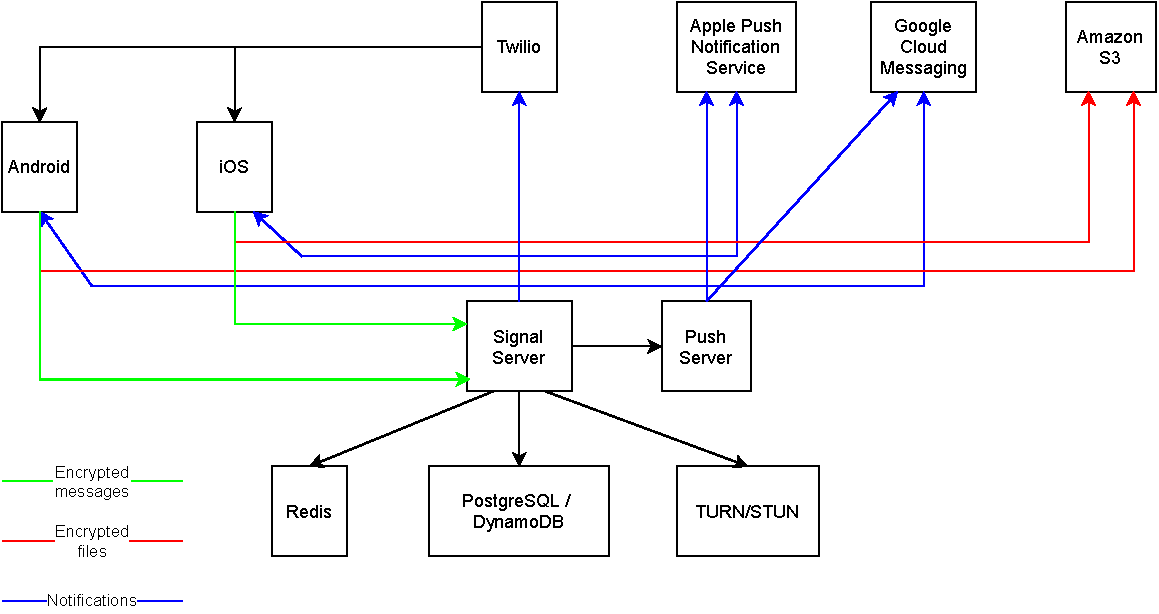
\includegraphics[width=\textwidth]{images/Architecture}
    \caption{Signal Server general architecture}
    \label{fig:signalarchitecture}
\end{figure}

The main differences between Signal 4.97 and Signal 6.13 are the use of DynamoDB as the main database instead of PostgreSQL and the use of AWS AppConfig\footnote{\url{https://docs.aws.amazon.com/appconfig/latest/userguide/what-is-appconfig.html}} to retrieve dynamic configuration data.

\section{Experiments\label{sec:experiments}}

The experiments I made can be divided into:
\begin{description}
    \item[steady load experiments] which use a base load slowly incremented over time in order to understand a measure of resilience of the architecture;
    \item[peak load experiments] which use a high load in a short time to understand the behavior of the architecture in this kind of conditions.   
\end{description}

For both of them I used a sequence of APIs call of Signal which reflects the ones made by an Android client in order to register a new account and in order to send a message from an account to another.

All the experiments have been executed both on Signal 4.97 and on Signal 6.13 in order to do a comparison between the results obtained with the two versions of the server.
The 4.97 version was used in production when an outage happened on the 15th January 2021, while the other version was the last available one when I started the server deployment.

In order to get the sequences of the calls made to the server from the load generator I used a real Android client, with a modified version of the code to log the calls made to the server in the correct order.



The following code is the modified method in the class \texttt{PushServiceSocket.java} to get the sequence of the calls which have been covered.

\begin{minted}[tabsize=2,breaklines]{java}
private String makeServiceRequest(String urlFragment, String method, String jsonBody, Map<String, String> headers, ResponseCodeHandler responseCodeHandler, Optional<UnidentifiedAccess> unidentifiedAccessKey)
    throws NonSuccessfulResponseCodeException, PushNetworkException
{
    System.out.println();
    System.out.println();
    System.out.println();
    for (Map.Entry<String, String> header : headers.entrySet()) {
        System.out.println("header-key: "+header.getKey());
        System.out.println("header-value: "+header.getValue());
    }
    if(urlFragment!=null) System.out.println("urlFragment: "+urlFragment);
    if(method!=null) System.out.println("method: "+method);
    if(jsonBody!=null) System.out.println("jsonBody: "+jsonBody);
    if(headers!=null) System.out.println("headers: "+headers.values().toString());
    if(unidentifiedAccessKey!=null) System.out.println("unidentifiedAccessKey: "+unidentifiedAccessKey.toString());
    System.out.println();
    System.out.println();
    System.out.println();
    ResponseBody responseBody = makeServiceBodyRequest(urlFragment, method, jsonRequestBody(jsonBody), headers, responseCodeHandler, unidentifiedAccessKey);
    try {
        return responseBody.string();
    } catch (IOException e) {
        throw new PushNetworkException(e);
    }
}
\end{minted}



Instead, in order to get the architectural components of Signal which are used from the previous calls I analyzed the source code of the 6.13 version of the Signal server, and I obtained some UML sequence diagrams that made it easier to understand the involved components\footnote{\url{https://drive.google.com/drive/folders/1G5RfzsEX8zLyv_yoq2h5FOEC-pLG0TPQ?usp=sharing}}.

More in detail on the design of the experiments, what I do is to create some situations of interests inspired to real scenarios.

Usually these kinds of test are designed by using real data of use, provided by logs or other sources and from configurations of the application itself.
In our experiments we have the components of the architecture, but we don't know any data relative to the load of the real system.

One of the possible options in this case is to ask some sample data to the people who manage the real application used in production.
I did not do this for time and privacy reasons. Signal is an application well known for the security of data of users who use it.
Obviously load data can be aggregated data, but maybe some of this kind of information can help in doing things that the owners of the application would not appreciate, so I decided to not ask them.

Another option is to verify the number of users who downloaded the application from the Play Store\footnote{\url{https://play.google.com/store}} and from the App Store\footnote{\url{https://www.apple.com/app-store}}, and to do an evaluation similar to the real situation on the number and on the behavior of the users.
I did not choose this option for time and cost motivations, it results very difficult for a master thesis project to rent on AWS the resources to simulate a real Signal server system.

This is the reason why we used a reduced scale system, which is easier to put under load, also with a limited number of requests, and which can be useful to give some interesting points about the weak points of the used architecture.

To load test the Signal server architecture we treated it as a black box system, in order to apply the possible results to other similar architectures.

Signal offers REST APIs which are used from its clients to exchange information with the server. We took into consideration a subset of those APIs, used for the creation of accounts and for sending messages.

As a consequence only some components of the architectures have been involved in the tests \parencite{read_2021,cocorada_2018}, such as the Dropwizard\footnote{\url{https://www.dropwizard.io/en/latest}} application itself, Redis\footnote{\url{https://redis.io}}, PostgreSQL\footnote{\url{https://www.postgresql.org}} and DynamoDB\footnote{\url{https://aws.amazon.com/dynamodb}} (only on the newer version of the Signal server).

\clearpage

What have been done in the thesis project is:
\begin{enumerate}
    \item extrapolate the components used by each API call from the Signal source code;
    \item find the components which are overloading the server;
    \item compare the two server versions between them.
\end{enumerate}

All the experiments are scaled down to the resources that I could afford.
For the server side I used the ones provided from the AWS free tier\footnote{\url{https://aws.amazon.com/free}}, with some expenses for the traffic and for DynamoDB resources.
For the client side I used my laptop.
These resources have a detailed description on the section \vref{sec:environment}.

With steady load we mean a load with a long duration in time which simulate the use of the application without relevant events.
It gets increased over time.

With peak load we mean a load with a short duration in time, which is used to simulate a particular event. For example, it can be the New Year's Eve when a lot of messages are sent in a limited period of time.

I give a more detailed description of these loads on the experimental section (see chapter \vref{sec:experimentalresults}).

\section{Issues left for future work\label{sec:uncovered}}

The following points are not covered from the thesis:
\begin{itemize}
    \item test of the architecture components used to send, receive and store multimedia contents different from simple messages;
    \item test of the components used for voice calls and video calls;
    \item test in a real world scale environment (only in a limited version);
    \item test with repetition from real world clients (only with load systems).
\end{itemize}
